\documentclass[a4paper]{article}

\usepackage[english]{babel}  % force American English hyphenation patterns
\usepackage[utf8x]{inputenc}  % unicode
\usepackage{graphicx}
\usepackage{wrapfig}
\usepackage{lipsum}  % generates filler text

\title{Package Example: wrapfig}
\author{writeLaTeX}

\begin{document}
\maketitle

\begin{wrapfigure}{R}{0.3\textwidth}
%\centering
  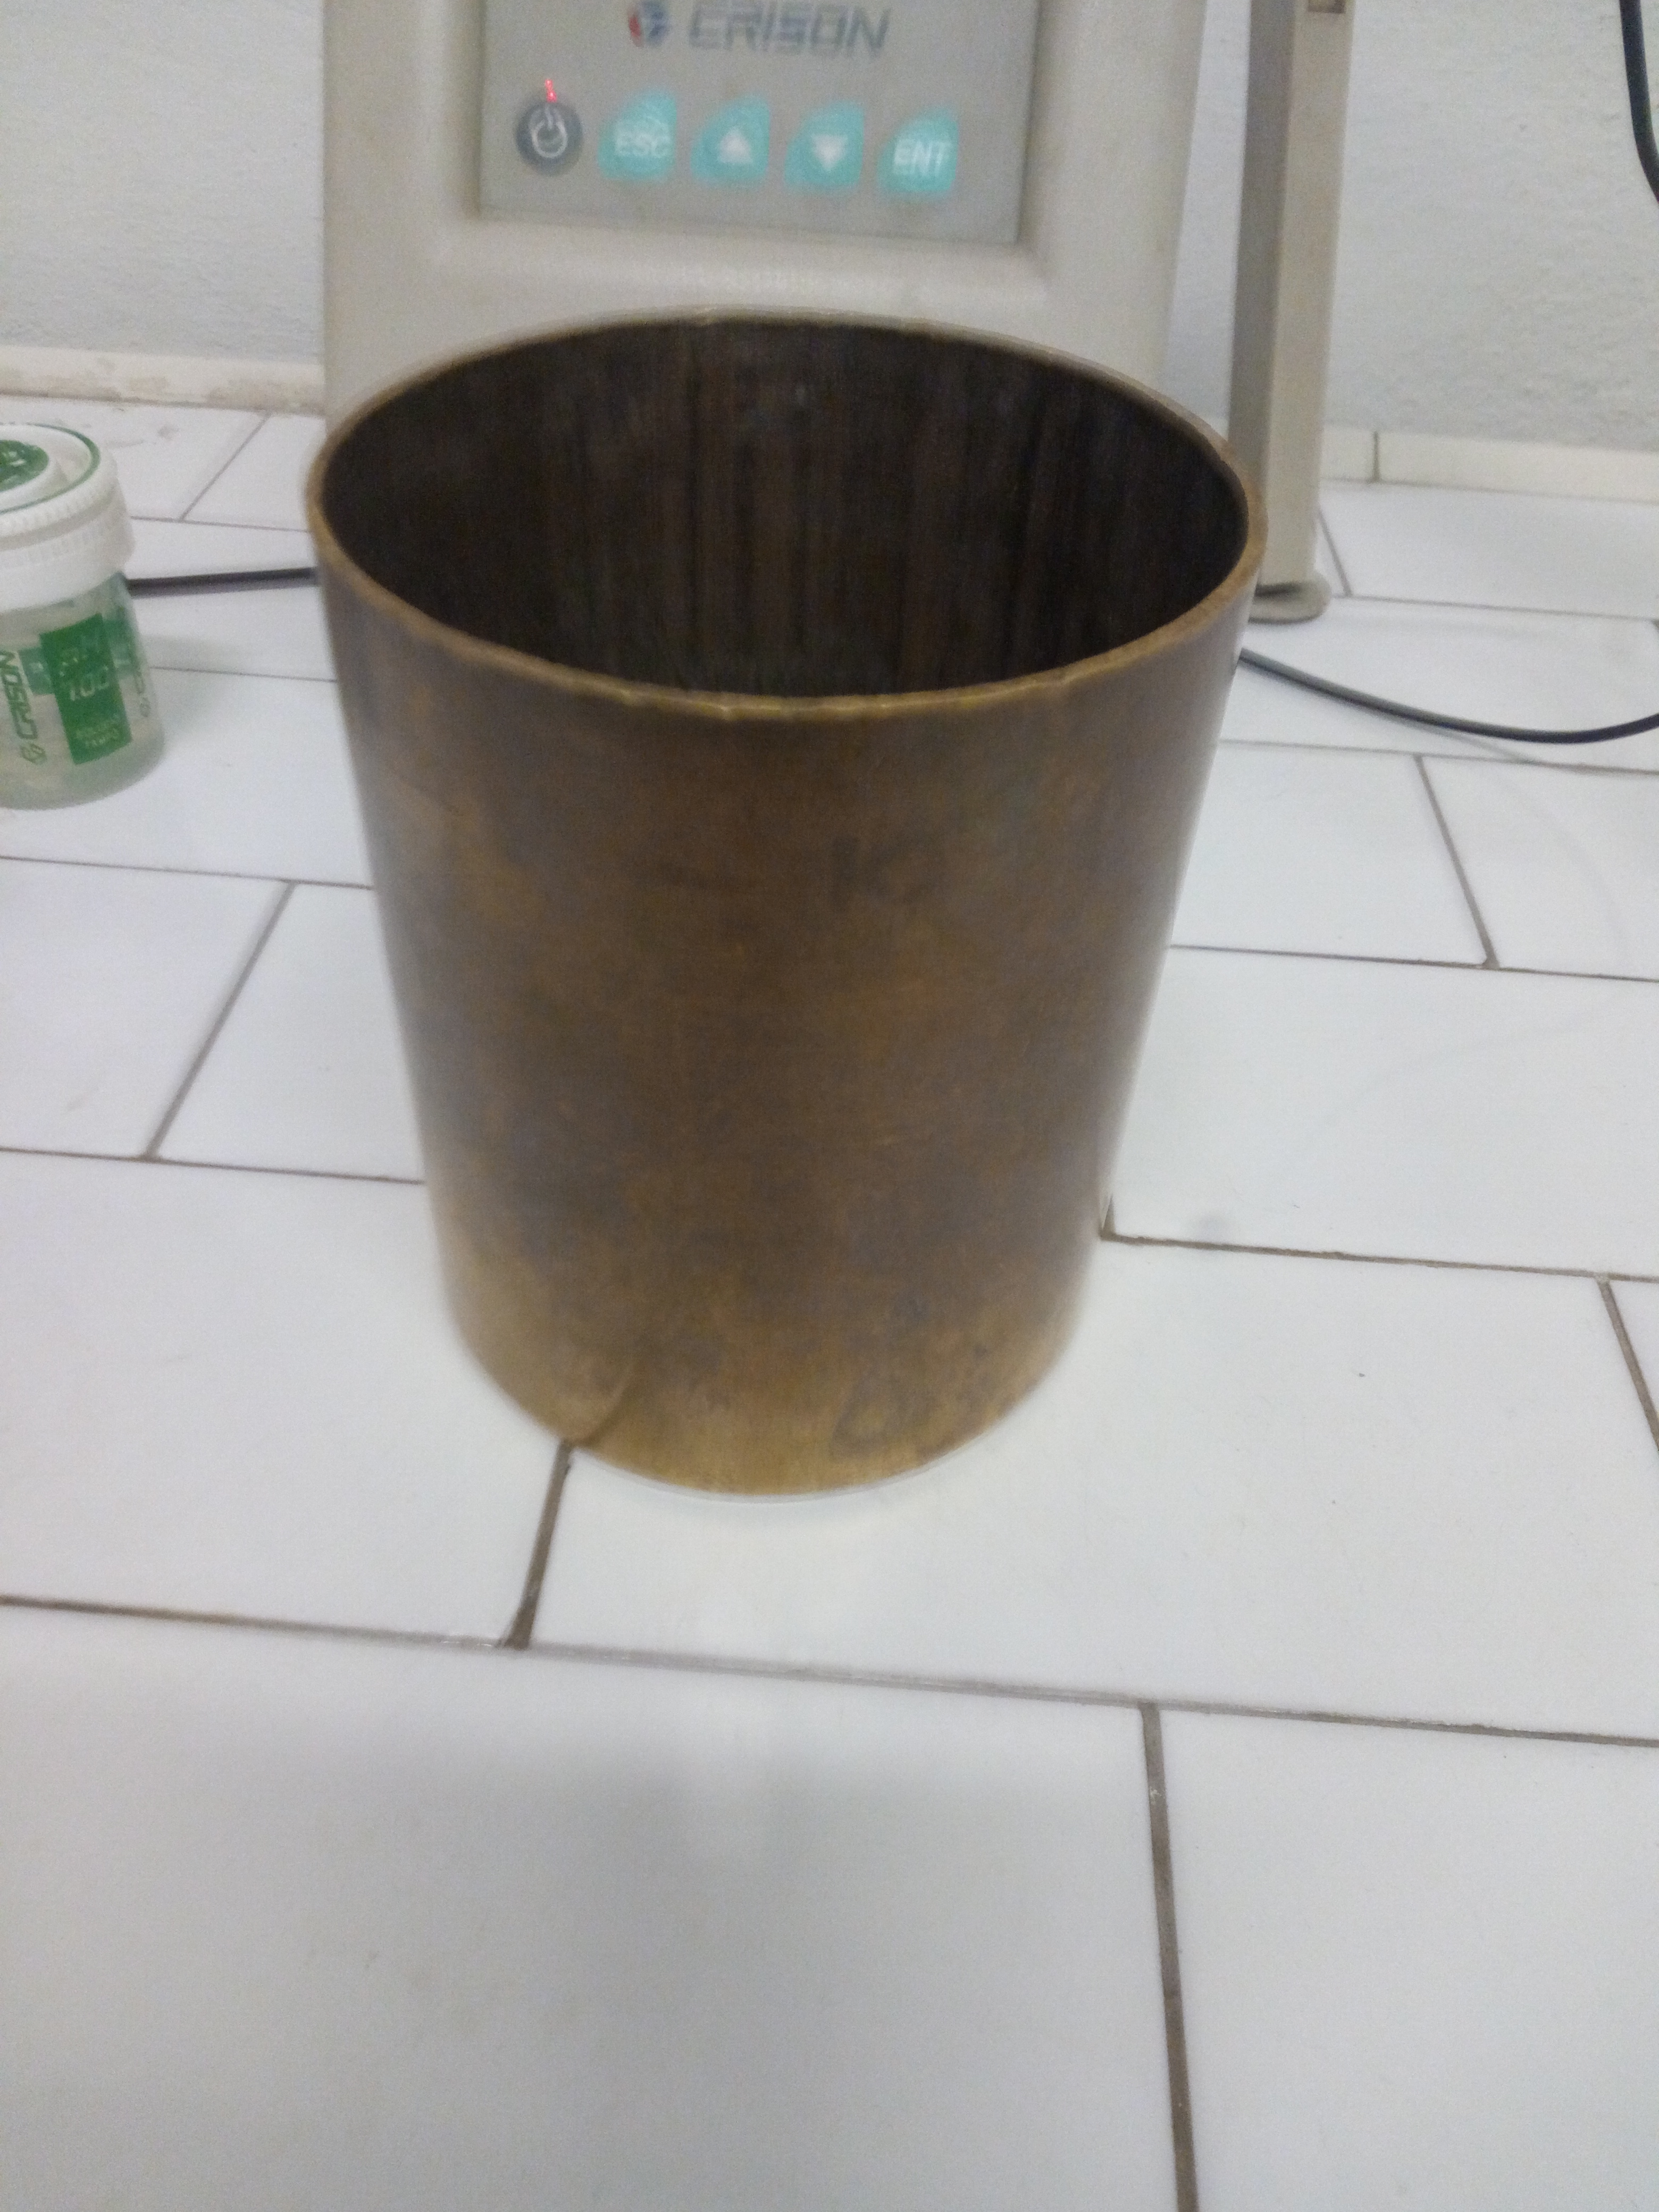
\includegraphics[width=0.5\textwidth]{../foto/cilindroOttone.jpeg}

  \caption[Cilindro in ottone usato per la misura della densità
  apparente: metodo \emph{Core}]{Cilindro in ottone utilizzato per
    prelevare i campioni da destinare all'analisi di densità
    apparente col metodo \emph{Core}.}
  \label{fig:cilindro}
\end{wrapfigure}

\lipsum[1]

\begin{wrapfigure}{L}{0.3\textwidth}
%\centering
  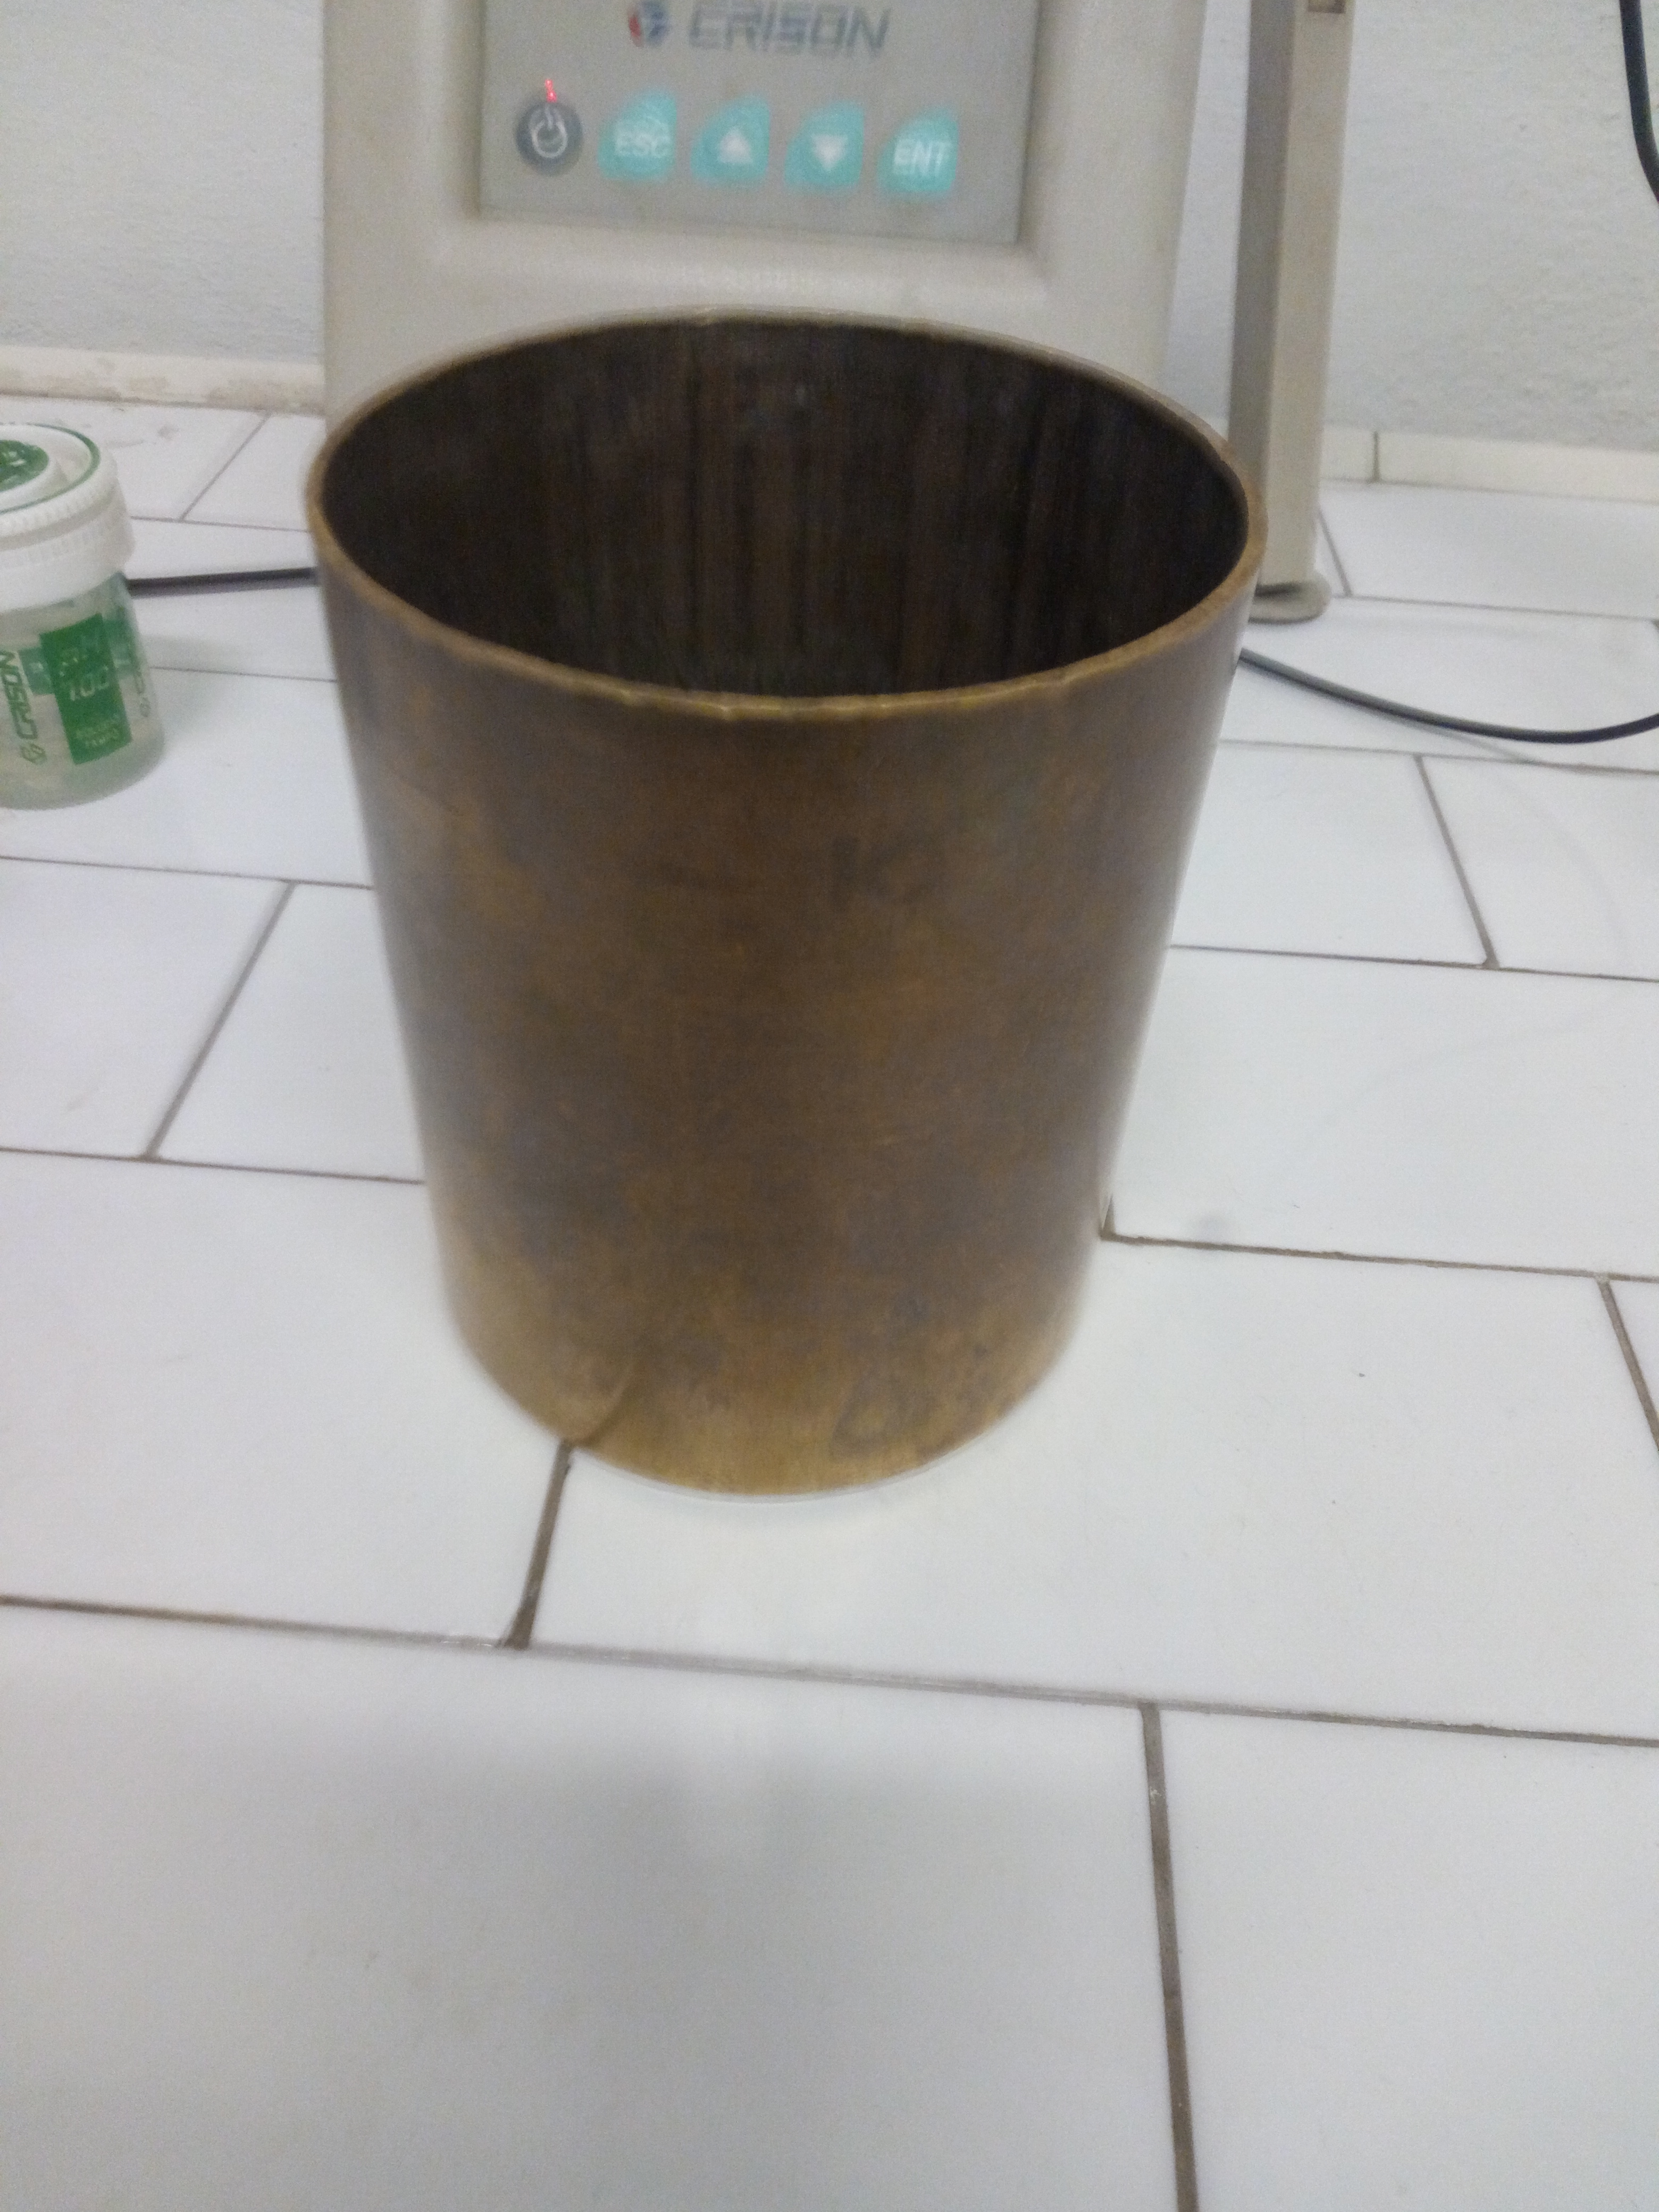
\includegraphics[width=0.5\textwidth]{../foto/cilindroOttone.jpeg}

  \caption[Cilindro in ottone usato per la misura della densità
  apparente: metodo \emph{Core}]{Cilindro in ottone utilizzato per
    prelevare i campioni da destinare all'analisi di densità
    apparente col metodo \emph{Core}.}
  \label{fig:cilindro}
\end{wrapfigure}

\lipsum[2-3]

\end{document}